%%%%%%%%%%%%%%%%%%%%%%%%%%%%%%%%%%%%%%%%%%%%%%%%%%%%%%%%%%%%%%%%%%%%%%%%%%%%%%%%
% CAPÍTULO 2
%%%%%%%%%%%%%%%%%%%%%%%%%%%%%%%%%%%%%%%%%%%%%%%%%%%%%%%%%%%%%%%%%%%%%%%%%%%%%%%%

\chapter{Título do capítulo}
\label{cap:capitulo-2}

Neste Capítulo ...

Acabei de colocar aqui uma figura que é a marca do NExT, veja-a Fig.~\ref{fig:next}.

\begin{figure}[h!]
  \begin{center}
    
\includegraphics[width=5cm]{next}
    \caption{Marca do NExT.}
    \label{fig:next}
  \end{center}
\end{figure}

Assim é que colocamos as figuras:

\begin{figure}[h!]
  \begin{center}
    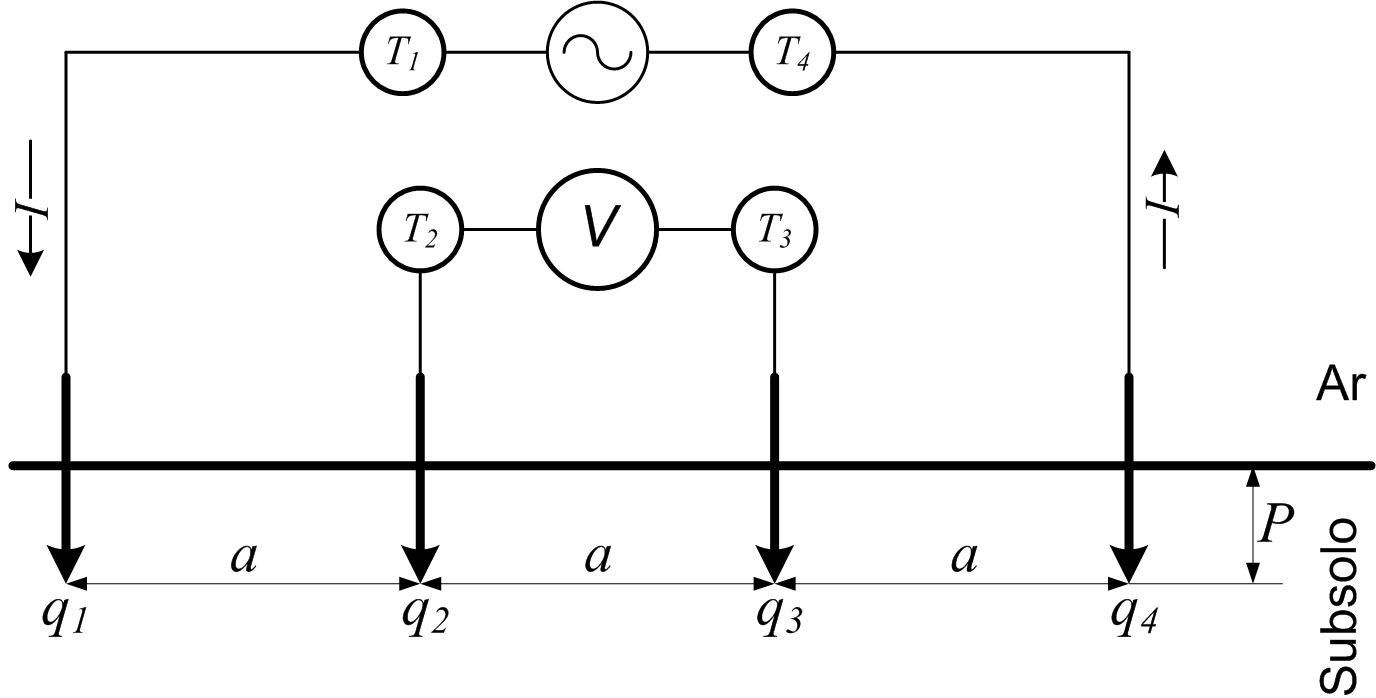
\includegraphics[width=.6\textwidth]{fig21}
    \caption{Método de \index{Wenner} Wenner.}
    \label{fig:metodo-wener}
  \end{center}
\end{figure}



Assim é que colocamos as equações:

\begin{equation}
  V_{q2} = \frac{\rho \cdot I}{4\pi}\left[\frac{1}{a} + \frac{1}{\sqrt{a^2 + (2P)^2}} - \frac{1}{2a} - \frac{1}{\sqrt{(2a)^2 + (2P)^2}}\right]
  \label{eq21}
\end{equation}

\begin{equation}
  V_{q3} = \frac{\rho \cdot I}{4\pi}\left[\frac{1}{2a} + \frac{1}{\sqrt{(2a)^2 + (2P)^2}} - \frac{1}{a} - \frac{1}{\sqrt{a^2 + (2P)^2}}\right]
  \label{eq22}
\end{equation}

Em (\ref{eq21}) e (\ref{eq22}), $a$ é a distância entre os \index{eletrodos} eletrodos, $P$ é a profundidade do eletrodo, $\rho$ a resistividade do solo. A diferença de potencial entre os pontos $q_2$ e $q_3$ é dada pela expressão (\ref{eq23}).

\begin{equation}
  V=V_{q2} - V_{q3} = \frac{\rho \cdot I}{4\pi}\left[\frac{1}{a} + \frac{1}{\sqrt{a^2 + (2P)^2}} - \frac{1}{\sqrt{(2a)^2 + (2P)^2}}\right]
  \label{eq23}
\end{equation}

Dividindo-se a diferença de potencial (\ref{eq23}) pela corrente $I$, obtém-se uma grandeza $R_m$ dimensionalmente igual a uma resistência elétrica \cite{bb14}.

\begin{equation}
  R_m = \frac{\rho}{4\pi}\left[\frac{1}{a} + \frac{1}{\sqrt{a^2 + 4P^2}} - \frac{1}{\sqrt{4a^2 + 4P^2}}\right]
  \label{eq24}
\end{equation}

Logo, isolando $\rho$ em (\ref{eq24}), tem-se a expressão para o cálculo da resistividade elétrica do solo.

\begin{equation}
  \rho = \frac{4 \pi a R_m}{1 + \frac{2a}{\sqrt{a^2 + 4P^2}} - \frac{2a}{\sqrt{4a^2 + 4P^2}}}
  \label{eq25}
\end{equation}

Para cada distância $a$ têm-se os valores de $V$ e $I$, medidos em campo e consequentemente obtém-se $R_m$ e, portanto pode-se calcular $\rho$ em (\ref{eq25}). Como o solo foi inicialmente considerado homogêneo, variando-se $a$, o valor de $R_m$ deve também variar de tal forma que $\rho$ permanece inalterado em (\ref{eq25}). Porém, na prática, o solo dificilmente se comporta com \index{homogeneidade} homogeneidade, e assim, o valor de $\rho$ calculado em (\ref{eq25}) deve variar com a distância $a$. A grandeza $\rho$ deixa de ter o significado de resistividade elétrica do solo, porém, contêm nos seus valores em função de $a$, propriedades que permitem identificar as diversas camadas homogêneas do solo.



%%% Local Variables:
%%% mode: latex
%%% TeX-master: "../main-dissertacao"
%%% coding: utf-8
%%% End:
